\section{Methodology}
\label{sec:Meth}

\begin{figure*}[t]
\centering
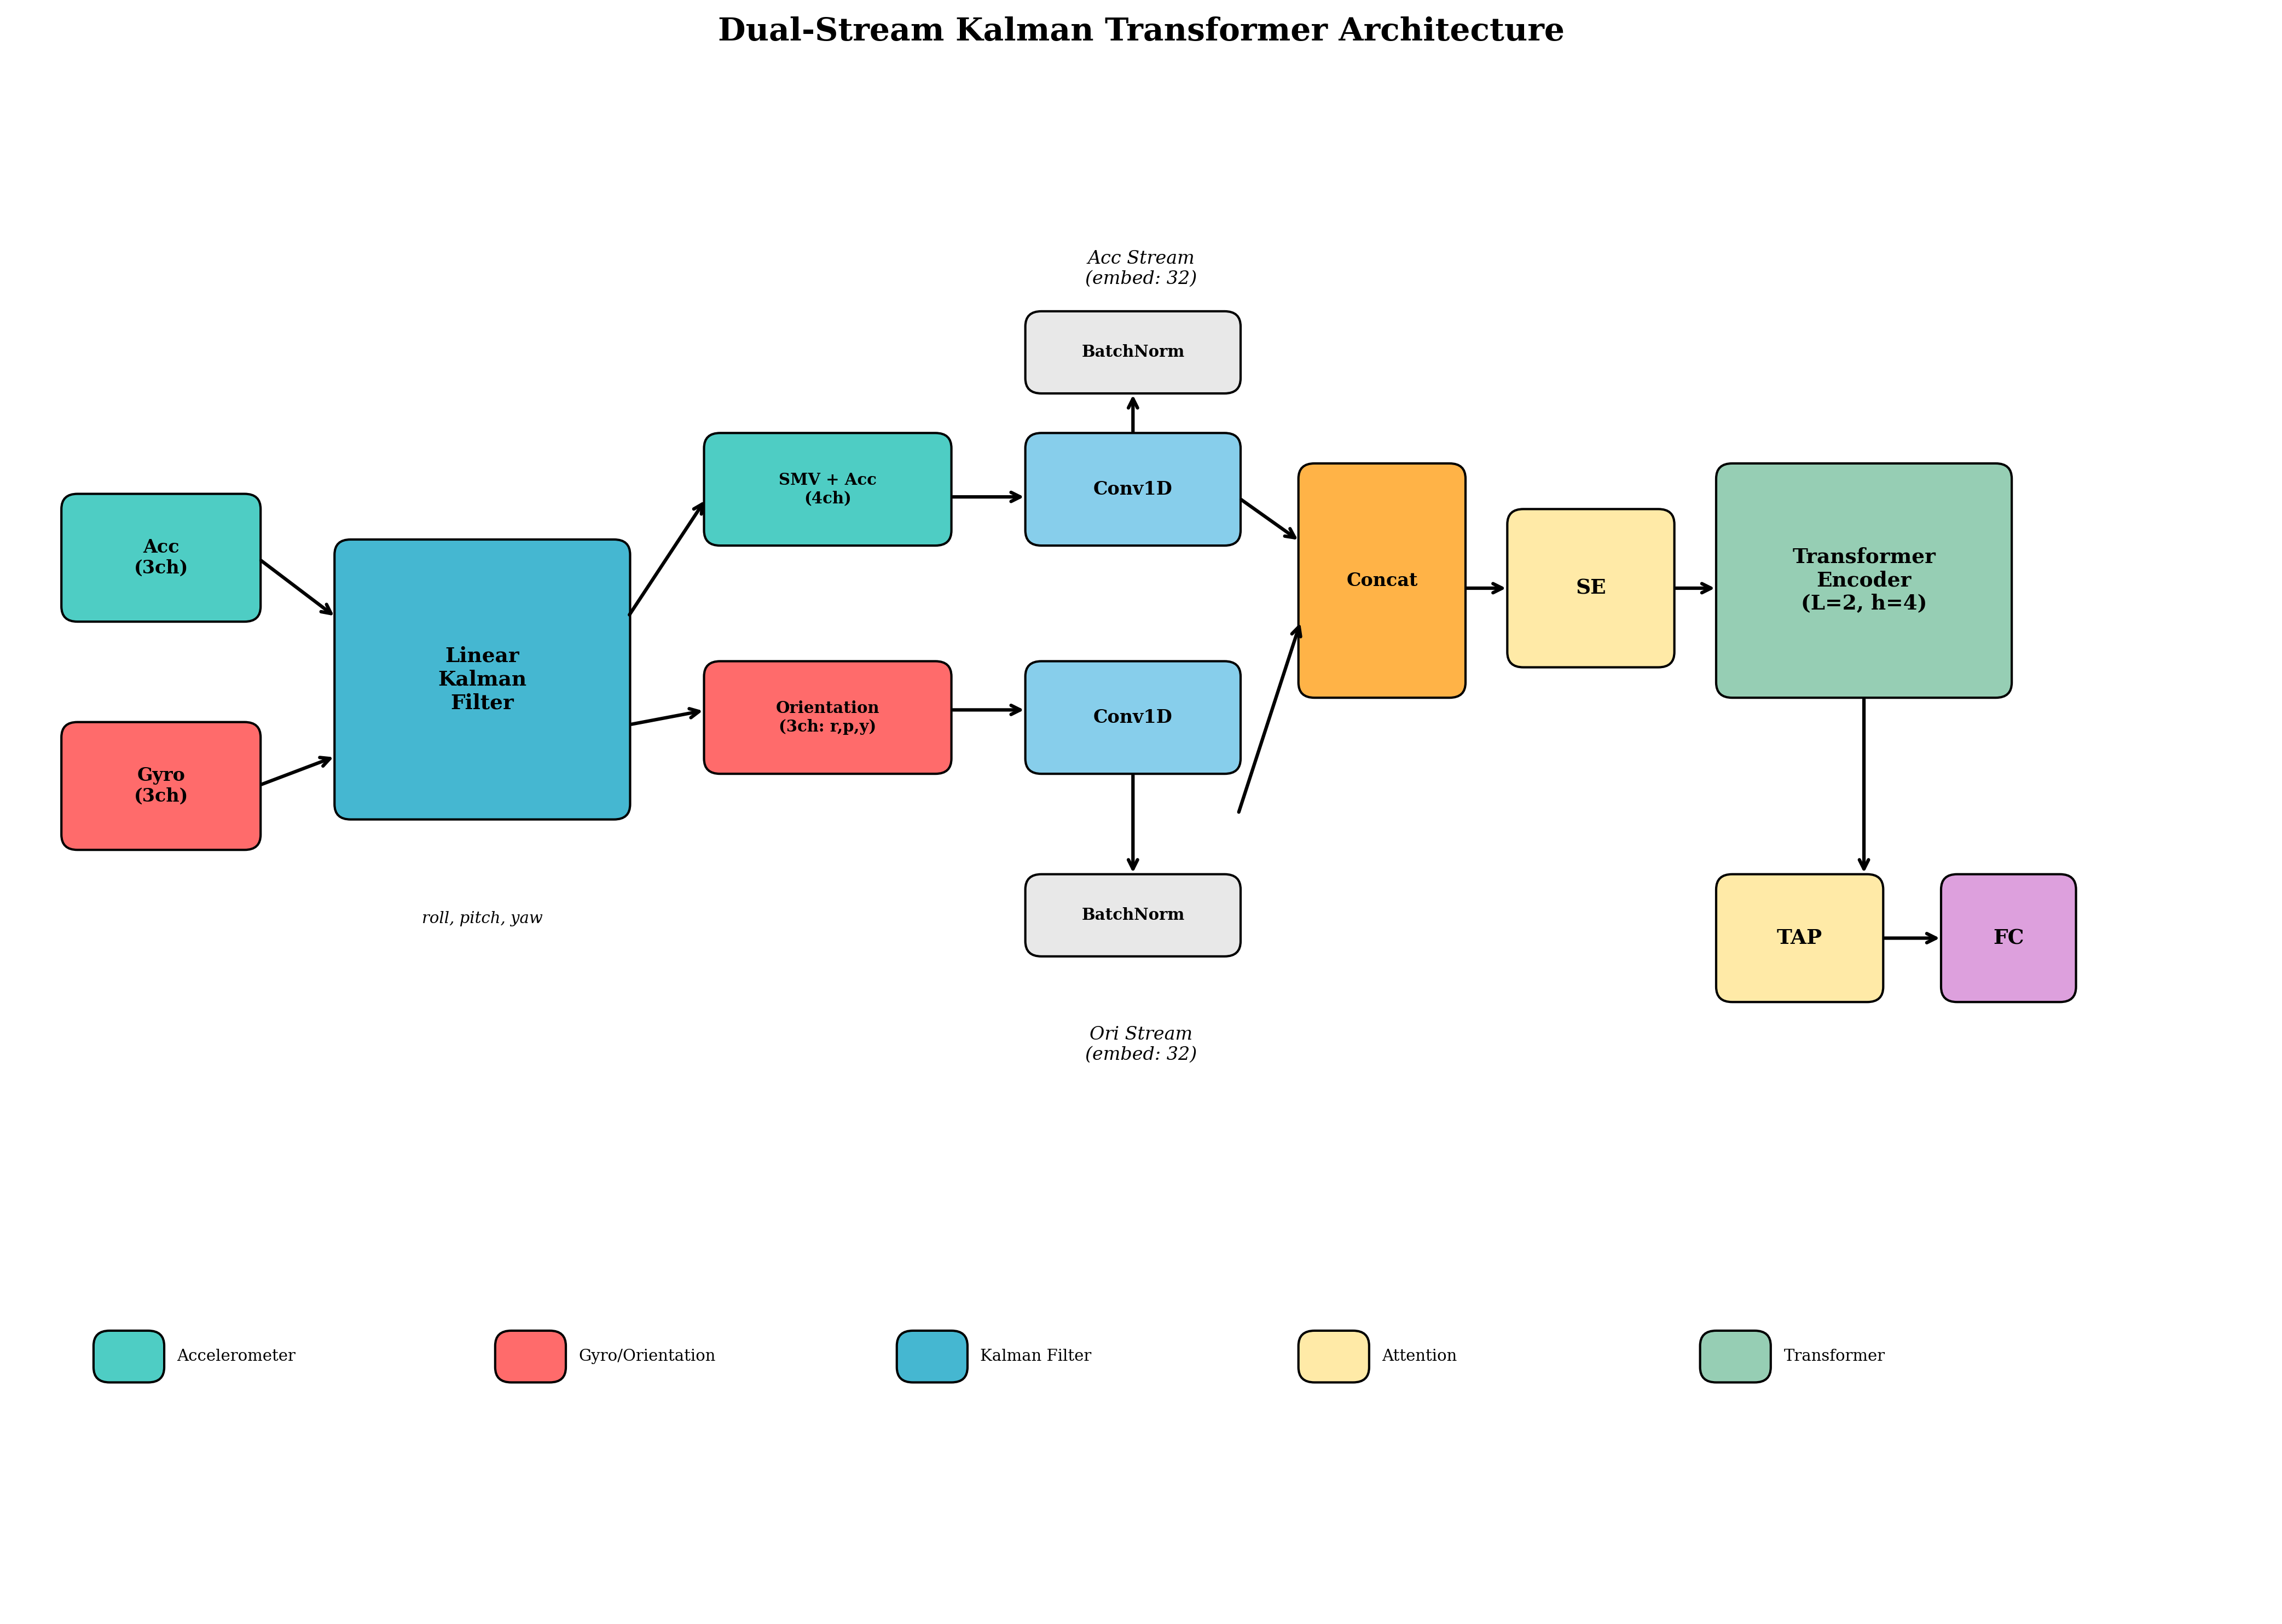
\includegraphics[width=0.95\textwidth]{figures/arch_dual_stream_kalman.png}
\caption{\textbf{Overview of Dual-Stream Kalman Transformer Architecture.} Raw accelerometer and gyroscope signals are fused through a Linear Kalman Filter to extract orientation estimates (roll, pitch, yaw). The resulting 7-channel features (SMV + accelerometer + orientation) are split into two parallel streams: (1) accelerometer stream processing motion magnitude, and (2) orientation stream processing body pose. Each stream undergoes Conv1D projection, BatchNorm, and Squeeze-Excitation (SE) attention before concatenation. The fused 64-dimensional features pass through a transformer encoder with temporal attention pooling (TAP) for fall/ADL classification. This architecture achieves 91.10\% F1 score on 21-fold LOSO cross-validation.}
\label{fig:overview}
\end{figure*}

\subsection{SmartFall System Architecture}
\label{sec:Arch}

\begin{figure}[t]
\centering
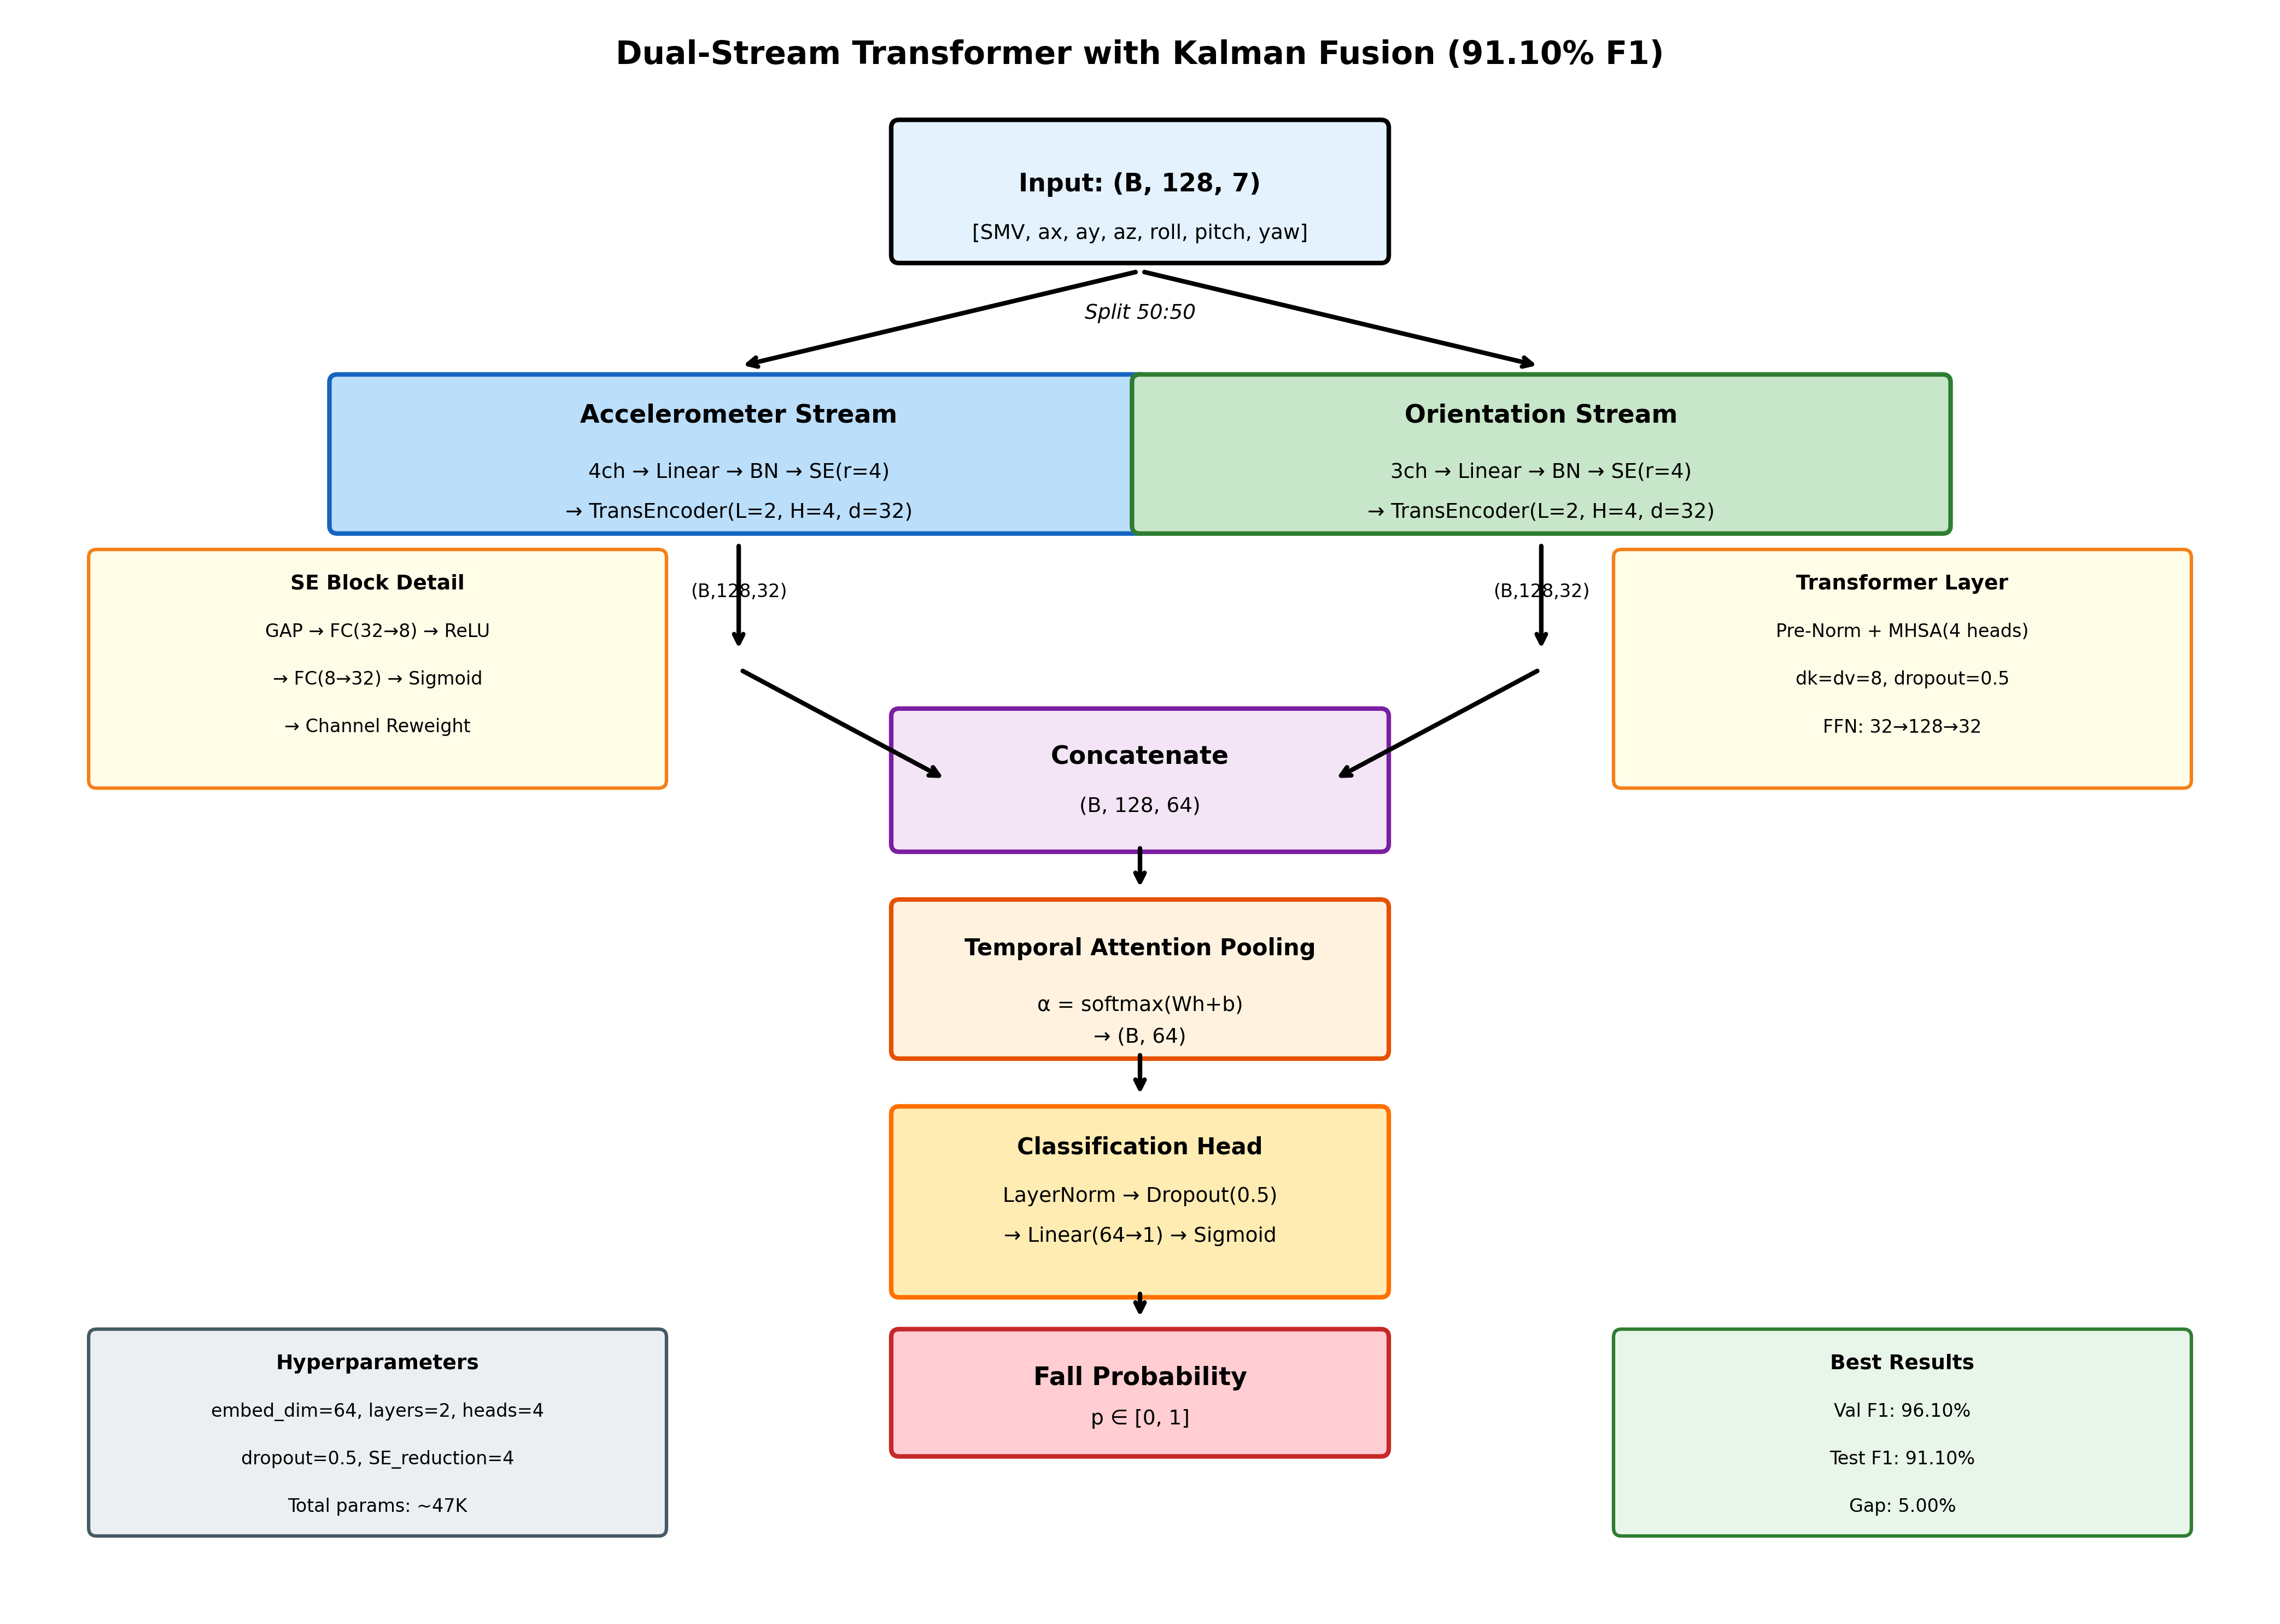
\includegraphics[width=\linewidth]{figures/architecture_diagram.png}
\caption{SmartFall system with Watch-Phone-based Architecture.}
\label{fig:Watch-Phone}
\end{figure}

Both single-stream and the dual-stream fall detection architectures are intended to be used on the wearable SmartFall system, which was developed in our lab \cite{ngu2022personalized, ngu2023p}. The overview of the system is shown in Figure~\ref{fig:Watch-Phone}. The three-layer SmartFall system is an AI-powered edge computing system designed to address the crucial need for efficient fall detection among older adults using a commodity-based wearable device. The watch is at the edge layer, the phone is in the middle layer, and the server for training and managing of the models is on the cloud. Central to its design is a user-centric approach that provides interaction with the fall detection system through a smartwatch interface, taking into account the challenges older adults face in handling multiple devices and their comfort with technology. The system can easily be configured with different versions of the fall detection model tailored to the individual user's motion pattern.

The system has been trialed among 19 older adults, structured to incorporate several vital software components, including:
\begin{itemize}
\item \textbf{Config Module:} This module manages the different versions of the fall detection model, personalization training strategy, and the selection of the cloud server, tailoring the system to individual user needs.

\item \textbf{Database Module:} This module handles the collection, storage, and cloud interactions of sensed data. It also provides for querying of the most optimized personalized models, ensuring users benefit from the best predictive tools available.

\item \textbf{Data Collector Module:} This module collects raw sensor data (accelerometer and gyroscope) sensed from the smartwatch. It can be configured to sense all available sensors provided by the watch's API and can handle various communication protocols, ensuring robust sensor data transfer.

\item \textbf{Prediction Module:} This module can be configured to use different machine learning models (such as ensemble recurrent neural networks (RNN/LSTM), single or dual stream transformer models, or multi-modal transformer models) to detect potential falls, aiming for timely and precise alerts to users.
\end{itemize}

This three-layer architecture is one of the most flexible architectures for wearable IoT applications as discussed in~\cite{NguIEEEIOT2017}.

\subsection{Linear Kalman Filter for Orientation Estimation}
\label{sec:KalmanFilter}

A key contribution of this work is the use of a Linear Kalman Filter to fuse accelerometer and gyroscope measurements into orientation estimates (roll, pitch, yaw). This section describes our implementation, which is based on classical Kalman filtering theory~\cite{kalman1960new}.

\subsubsection{State Space Formulation}

We define the state vector as:
\begin{equation}
\mathbf{x} = \begin{bmatrix} \phi & \theta & \psi & \dot{\phi} & \dot{\theta} & \dot{\psi} \end{bmatrix}^T
\end{equation}
where $\phi$, $\theta$, $\psi$ represent roll, pitch, and yaw angles respectively, and $\dot{\phi}$, $\dot{\theta}$, $\dot{\psi}$ are the corresponding angular rates.

\subsubsection{State Transition Model}

The state transition follows a constant angular velocity model:
\begin{equation}
\mathbf{x}_{k} = \mathbf{F} \mathbf{x}_{k-1} + \mathbf{w}_{k}
\end{equation}
where the state transition matrix $\mathbf{F}$ is:
\begin{equation}
\mathbf{F} = \begin{bmatrix}
1 & 0 & 0 & \Delta t & 0 & 0 \\
0 & 1 & 0 & 0 & \Delta t & 0 \\
0 & 0 & 1 & 0 & 0 & \Delta t \\
0 & 0 & 0 & 1 & 0 & 0 \\
0 & 0 & 0 & 0 & 1 & 0 \\
0 & 0 & 0 & 0 & 0 & 1
\end{bmatrix}
\end{equation}
and $\mathbf{w}_k \sim \mathcal{N}(0, \mathbf{Q})$ is the process noise with covariance:
\begin{equation}
\mathbf{Q} = \text{diag}(Q_{\text{ori}}, Q_{\text{ori}}, Q_{\text{ori}}, Q_{\text{rate}}, Q_{\text{rate}}, Q_{\text{rate}})
\end{equation}

In our implementation, we use $Q_{\text{ori}} = 0.005$ rad$^2$ and $Q_{\text{rate}} = 0.01$ (rad/s)$^2$.

\subsubsection{Observation Model}

The observation vector consists of roll and pitch derived from accelerometer measurements and angular rates from the gyroscope:
\begin{equation}
\mathbf{z} = \begin{bmatrix} \phi_{\text{acc}} & \theta_{\text{acc}} & \omega_x & \omega_y & \omega_z \end{bmatrix}^T
\end{equation}

Roll and pitch are estimated from the accelerometer using the gravity reference:
\begin{align}
\phi_{\text{acc}} &= \arctan\left(\frac{a_y}{a_z}\right) \\
\theta_{\text{acc}} &= \arctan\left(\frac{-a_x}{\sqrt{a_y^2 + a_z^2}}\right)
\end{align}
where $a_x$, $a_y$, $a_z$ are the accelerometer readings. Note that yaw is not directly observable without a magnetometer.

The observation matrix $\mathbf{H}$ maps the state to observations:
\begin{equation}
\mathbf{H} = \begin{bmatrix}
1 & 0 & 0 & 0 & 0 & 0 \\
0 & 1 & 0 & 0 & 0 & 0 \\
0 & 0 & 0 & 1 & 0 & 0 \\
0 & 0 & 0 & 0 & 1 & 0 \\
0 & 0 & 0 & 0 & 0 & 1
\end{bmatrix}
\end{equation}

The measurement noise covariance is:
\begin{equation}
\mathbf{R} = \text{diag}(R_{\text{acc}}, R_{\text{acc}}, R_{\text{gyro}}, R_{\text{gyro}}, R_{\text{gyro}})
\end{equation}
with tuned values $R_{\text{acc}} = 0.05$ rad$^2$ and $R_{\text{gyro}} = 0.1$ (rad/s)$^2$.

\subsubsection{Kalman Filter Equations}

The filter operates in two steps per timestep:

\textbf{Prediction Step:}
\begin{align}
\hat{\mathbf{x}}_{k|k-1} &= \mathbf{F} \hat{\mathbf{x}}_{k-1|k-1} \\
\mathbf{P}_{k|k-1} &= \mathbf{F} \mathbf{P}_{k-1|k-1} \mathbf{F}^T + \mathbf{Q}
\end{align}

\textbf{Update Step:}
\begin{align}
\mathbf{y}_k &= \mathbf{z}_k - \mathbf{H} \hat{\mathbf{x}}_{k|k-1} & \text{(Innovation)} \\
\mathbf{S}_k &= \mathbf{H} \mathbf{P}_{k|k-1} \mathbf{H}^T + \mathbf{R} & \text{(Innovation covariance)} \\
\mathbf{K}_k &= \mathbf{P}_{k|k-1} \mathbf{H}^T \mathbf{S}_k^{-1} & \text{(Kalman gain)} \\
\hat{\mathbf{x}}_{k|k} &= \hat{\mathbf{x}}_{k|k-1} + \mathbf{K}_k \mathbf{y}_k & \text{(State update)} \\
\mathbf{P}_{k|k} &= (\mathbf{I} - \mathbf{K}_k \mathbf{H}) \mathbf{P}_{k|k-1} & \text{(Covariance update)}
\end{align}

For numerical stability, we use the Joseph form for covariance update:
\begin{equation}
\mathbf{P}_{k|k} = (\mathbf{I} - \mathbf{K}_k \mathbf{H}) \mathbf{P}_{k|k-1} (\mathbf{I} - \mathbf{K}_k \mathbf{H})^T + \mathbf{K}_k \mathbf{R} \mathbf{K}_k^T
\end{equation}

Angle wrapping to $[-\pi, \pi]$ is applied after each update to handle angle discontinuities.

\subsubsection{Output Features}

The final feature vector for each timestep consists of 7 channels:
\begin{equation}
\mathbf{f} = \begin{bmatrix} \text{SMV} & a_x & a_y & a_z & \phi & \theta & \psi \end{bmatrix}^T
\end{equation}
where SMV (Signal Magnitude Vector) is computed as $\text{SMV} = \sqrt{a_x^2 + a_y^2 + a_z^2}$.

This representation replaces the raw gyroscope signals ($\omega_x$, $\omega_y$, $\omega_z$) with physically interpretable orientation angles, providing the fall detection model with a more meaningful feature space.

\subsection{Kalman Filter Design Validation}
\label{sec:KalmanValidation}

The use of a Linear Kalman Filter for IMU orientation estimation raises several theoretical concerns that merit careful examination. We address each concern with empirical validation specific to our fall detection application.

\subsubsection{Gravity Assumption During Fall Impacts}

The accelerometer-derived roll and pitch observations (Equations 7--8) assume that measured acceleration is dominated by gravity ($\|\mathbf{a}\| \approx 9.81$ m/s$^2$). During fall impacts, linear acceleration can spike to 20--30 m/s$^2$, potentially contaminating the gravity reference and introducing systematic orientation errors precisely when accurate estimates matter most.

We argue this limitation has minimal impact on our system for two reasons. First, our classification operates on 128-sample windows (4.27 seconds at 30 Hz). The fall impact phase typically spans 3--9 samples (0.1--0.3 seconds), representing less than 7\% of each window. During the remaining 93\%+ of the window, the gravity assumption holds. Second, when the filter produces orientation ``errors'' during impact, these artifacts become learnable fall signatures---the sequence of [stable orientation $\rightarrow$ discontinuity $\rightarrow$ new stable orientation] is itself discriminative.

To validate this empirically, we implemented adaptive measurement noise gating that inflates $R_{\text{acc}}$ when $\|\mathbf{a}\| > 1.5g$:
\begin{equation}
R_{\text{acc}}^{\text{adaptive}} = \begin{cases}
R_{\text{acc}} \cdot \left(\frac{\|\mathbf{a}\|}{g}\right)^2 & \text{if } \|\mathbf{a}\| > 1.5g \\
R_{\text{acc}} & \text{otherwise}
\end{cases}
\end{equation}

Table~\ref{tab:adaptive_racc} shows this theoretically-motivated enhancement produced no improvement ($\Delta = -0.02\%$ F1), confirming that constant measurement noise is sufficient for our application.

\begin{table}[htbp]
\centering
\caption{Adaptive Measurement Noise Ablation (21-fold LOSO-CV)}
\label{tab:adaptive_racc}
\begin{tabular}{@{}lcc@{}}
\toprule
\textbf{Configuration} & \textbf{Test F1 (\%)} & \textbf{$\Delta$} \\
\midrule
Constant $R_{\text{acc}} = 0.05$ (baseline) & 90.65 & --- \\
Adaptive $R_{\text{acc}}$ (threshold 1.5$g$) & 90.63 & $-0.02$ \\
\bottomrule
\end{tabular}
\end{table}

\subsubsection{Yaw Observability Without Magnetometer}

Without a magnetometer, yaw ($\psi$) lacks an absolute reference and can only be estimated through gyroscope integration, which accumulates drift from sensor bias (typically 0.1--1.0$^\circ$/s in consumer MEMS gyroscopes). Reviewers may question whether yaw-derived features generalize or merely capture device-specific drift artifacts.

Three factors mitigate this concern in our system. First, our short 4.27-second windows limit maximum drift to $1.0^\circ/\text{s} \times 4.27\text{s} = 4.27^\circ$, which is negligible compared to fall rotation magnitudes (90--180$^\circ$ for lateral and rotation falls). Second, the Kalman filter is re-initialized for each window, preventing inter-window drift accumulation. Third, fall detection requires distinguishing \textit{relative} yaw dynamics (rotation falls exhibit high yaw rate; backward falls exhibit minimal yaw change), not absolute heading.

To quantify yaw's contribution, we conducted an ablation removing yaw from the feature set (Table~\ref{tab:yaw_ablation}). The 1.25\% F1 degradation confirms that yaw provides discriminative information despite theoretical drift concerns.

\begin{table}[htbp]
\centering
\caption{Yaw Channel Ablation (21-fold LOSO-CV)}
\label{tab:yaw_ablation}
\begin{tabular}{@{}lcc@{}}
\toprule
\textbf{Configuration} & \textbf{Test F1 (\%)} & \textbf{$\Delta$} \\
\midrule
6-channel (no yaw): [SMV, $\mathbf{a}$, $\phi$, $\theta$] & 89.40 & $-1.25$ \\
7-channel (with yaw): [SMV, $\mathbf{a}$, $\phi$, $\theta$, $\psi$] & 90.65 & --- \\
\bottomrule
\end{tabular}
\end{table}

\subsubsection{Gyroscope Bias Estimation}

Standard practice in IMU orientation estimation is to augment the filter state with gyroscope bias terms, enabling online bias correction. Our Linear Kalman Filter does not estimate bias, which theoretically allows bias-induced drift to corrupt orientation estimates.

We compared our 6-dimensional Linear Kalman Filter against a 9-dimensional Extended Kalman Filter (EKF) with explicit bias estimation:
\begin{equation}
\mathbf{x}_{\text{EKF}} = \begin{bmatrix} \phi & \theta & \psi & \dot{\phi} & \dot{\theta} & \dot{\psi} & b_{\omega_x} & b_{\omega_y} & b_{\omega_z} \end{bmatrix}^T
\end{equation}

Counter-intuitively, the EKF with bias estimation performed \textit{worse} than the simpler Linear Kalman Filter (Table~\ref{tab:bias_ablation}). We attribute this to three factors: (1) bias is only observable during quasi-static periods, which are rare in 4.27-second windows containing falls; (2) the EKF attempts to estimate bias from insufficient data, introducing estimation noise; (3) the neural network learns to compensate for consistent filter behavior, whereas unstable EKF estimates add variance the network cannot model.

\begin{table}[htbp]
\centering
\caption{Bias Estimation Ablation (21-fold LOSO-CV)}
\label{tab:bias_ablation}
\begin{tabular}{@{}lccc@{}}
\toprule
\textbf{Filter} & \textbf{Bias Est.} & \textbf{Test F1 (\%)} & \textbf{$\Delta$} \\
\midrule
Linear Kalman (6D) & No & 90.91 & $+0.26$ \\
Extended Kalman (9D) & Yes & 88.89 & $-2.02$ \\
\bottomrule
\end{tabular}
\end{table}

This finding demonstrates that simpler is better for short-window fall detection: the 4.27-second duration bounds bias-induced drift to levels ($<5^\circ$) that are less harmful than EKF estimation noise under dynamic conditions.

\subsubsection{Euler Angle Representation}

Euler angles can exhibit discontinuities at angle boundaries and ill-conditioning near gimbal lock ($\theta = \pm 90^\circ$). We mitigate discontinuities through angle wrapping:
\begin{equation}
\text{wrap}(\alpha) = \text{atan2}(\sin(\alpha), \cos(\alpha))
\end{equation}
applied after each Kalman update. Gimbal lock is rare in fall scenarios---it requires the subject to be oriented nearly vertical (looking straight up/down)---and our empirical results (91.10\% F1) demonstrate robust performance despite this theoretical limitation.

\subsection{Feature Representation and Units}
\label{sec:FeatureUnits}

To ensure reproducibility and prevent unit-related errors, we precisely define all feature channels and their transformations.

\subsubsection{Input Feature Specification}

Table~\ref{tab:feature_units} specifies the 7-channel Kalman-fused feature vector used as model input.

\begin{table}[htbp]
\centering
\caption{Feature Channel Specification}
\label{tab:feature_units}
\resizebox{\columnwidth}{!}{%
\begin{tabular}{@{}clccc@{}}
\toprule
\textbf{Ch.} & \textbf{Feature} & \textbf{Units} & \textbf{Range} & \textbf{Normalization} \\
\midrule
0 & SMV ($\|\mathbf{a}\|$) & m/s$^2$ & $[0, 35]$ & StandardScaler \\
1 & Accelerometer $a_x$ & m/s$^2$ & $[-20, 20]$ & StandardScaler \\
2 & Accelerometer $a_y$ & m/s$^2$ & $[-20, 20]$ & StandardScaler \\
3 & Accelerometer $a_z$ & m/s$^2$ & $[-20, 20]$ & StandardScaler \\
4 & Roll $\phi$ & radians & $[-\pi, \pi]$ & None (raw) \\
5 & Pitch $\theta$ & radians & $[-\frac{\pi}{2}, \frac{\pi}{2}]$ & None (raw) \\
6 & Yaw $\psi$ & radians & $[-\pi, \pi]$ & None (raw) \\
\bottomrule
\end{tabular}%
}
\end{table}

Raw gyroscope measurements (degrees/s) are converted to radians/s prior to Kalman filtering. Orientation angles follow the ZYX (aerospace) Euler convention with rotation order $R = R_z(\psi) \cdot R_y(\theta) \cdot R_x(\phi)$.

\subsubsection{Channel-Aware Normalization Rationale}

We apply z-score normalization only to accelerometer channels (0--3), preserving orientation angles in raw radians. This design choice reflects the different characteristics of each modality:

\begin{itemize}
\item \textbf{Accelerometer channels}: Unbounded during falls (can spike to 30+ m/s$^2$), requiring normalization to prevent scale domination in the neural network.
\item \textbf{Orientation channels}: Already bounded ($\pm\pi$ radians) with physical meaning---$\phi = 0$ indicates level orientation, $\phi = -\pi/2$ indicates lying on one's side. Normalization would destroy this semantic information.
\end{itemize}

This channel-aware approach improves test F1 by +0.23\% compared to normalizing all channels together (Section~\ref{sec:channel_aware_norm}).

\subsection{Dual-Stream Transformer Architecture}
\label{sec:DualStream}

Our architecture processes Kalman-fused features through parallel encoder streams, leveraging Squeeze-and-Excitation (SE) attention for channel weighting and Temporal Attention Pooling (TAP) for sequence aggregation (Figure~\ref{fig:overview}). For comparison, Figure~\ref{fig:single_stream} shows the single-stream baseline that achieves 89.49\% F1 but suffers from noisy gyroscope signals corrupting accelerometer features.

\begin{figure}[htbp]
\centering
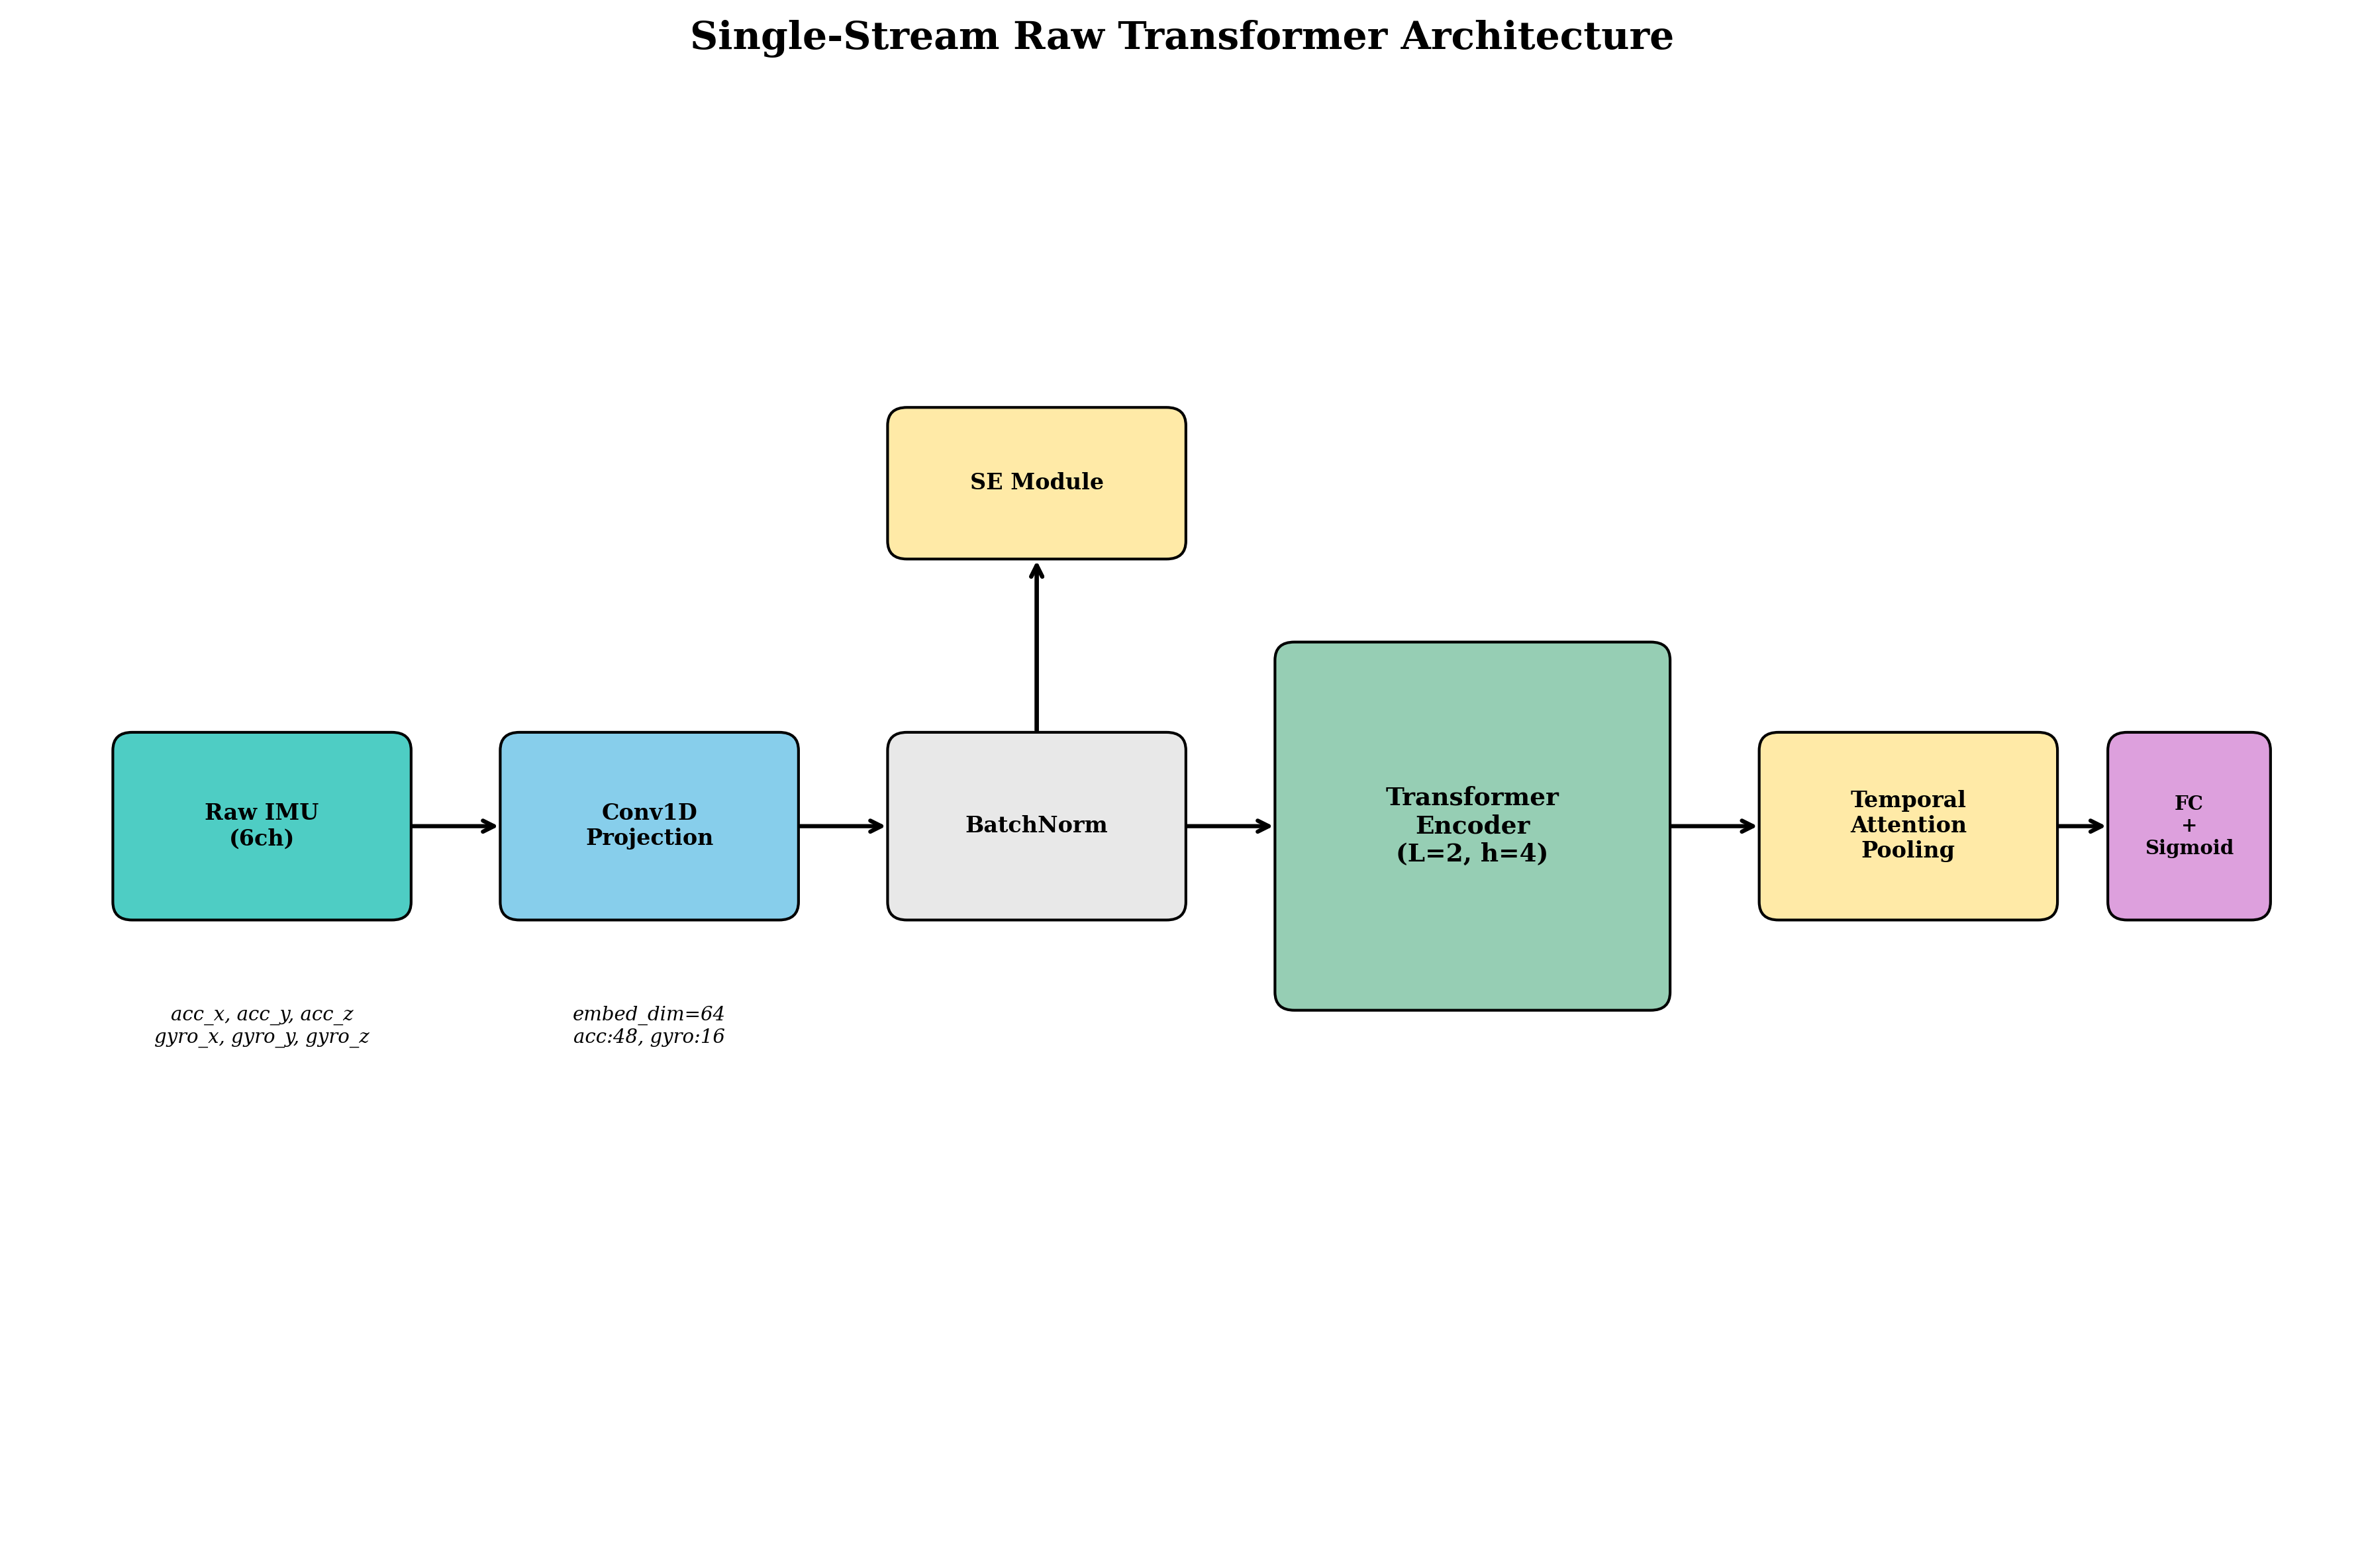
\includegraphics[width=0.85\columnwidth]{figures/arch_single_stream.png}
\caption{Single-stream baseline architecture processing raw 6-channel IMU data through a shared embedding space.}
\label{fig:single_stream}
\end{figure}

\subsubsection{Architecture Specification}

Table~\ref{tab:architecture} summarizes the layer-by-layer configuration achieving 91.10\% test F1 with only $\sim$47K parameters.

\begin{table}[htbp]
\centering
\caption{Dual-Stream Transformer Architecture}
\label{tab:architecture}
\resizebox{\columnwidth}{!}{%
\begin{tabular}{@{}llc@{}}
\toprule
\textbf{Layer} & \textbf{Operation} & \textbf{Output Shape} \\
\midrule
\multicolumn{3}{l}{\textit{Input \& Split}} \\
Input & Kalman features & $(B, T, 7)$ \\
Split & $\mathbf{X}_{\text{acc}} = \mathbf{X}_{[:,0:4]}$, $\mathbf{X}_{\text{ori}} = \mathbf{X}_{[:,4:7]}$ & $(B,T,4)$, $(B,T,3)$ \\
\midrule
\multicolumn{3}{l}{\textit{Stream Processing ($\times 2$)}} \\
Projection & $\mathbf{H} = \text{Conv1D}(\mathbf{X}, d_{\text{emb}}=32)$ & $(B, T, 32)$ \\
Normalize & $\hat{\mathbf{H}} = \text{BatchNorm}(\mathbf{H})$ & $(B, T, 32)$ \\
SE Attention & $\tilde{\mathbf{H}} = \hat{\mathbf{H}} \odot \sigma(\text{MLP}(\text{GAP}(\hat{\mathbf{H}})))$ & $(B, T, 32)$ \\
Transformer & $\mathbf{Z} = \text{TransEnc}(\tilde{\mathbf{H}}; L{=}2, h{=}4)$ & $(B, T, 32)$ \\
\midrule
\multicolumn{3}{l}{\textit{Fusion \& Classification}} \\
Concatenate & $\mathbf{F} = [\mathbf{Z}_{\text{acc}}; \mathbf{Z}_{\text{ori}}]$ & $(B, T, 64)$ \\
TAP & $\mathbf{c} = \sum_t \alpha_t \mathbf{F}_t$, \; $\alpha = \text{softmax}(\mathbf{W}\mathbf{F})$ & $(B, 64)$ \\
Classifier & $\hat{y} = \sigma(\mathbf{W}_c \cdot \text{LN}(\mathbf{c}))$ & $(B, 1)$ \\
\bottomrule
\end{tabular}%
}
\vspace{1mm}
\scriptsize
$B$: batch size, $T{=}128$: sequence length, $L$: transformer layers, $h$: attention heads
\end{table}

\subsubsection{Squeeze-and-Excitation (SE) Module}

The SE module~\cite{hu2018squeeze} learns channel-wise attention weights through global context aggregation:
\begin{equation}
\text{SE}(\mathbf{H}) = \mathbf{H} \odot \sigma\left(\mathbf{W}_2 \cdot \text{ReLU}(\mathbf{W}_1 \cdot \text{GAP}(\mathbf{H}))\right)
\end{equation}
where $\text{GAP}(\cdot)$ denotes global average pooling, $\mathbf{W}_1 \in \mathbb{R}^{d/r \times d}$ and $\mathbf{W}_2 \in \mathbb{R}^{d \times d/r}$ with reduction ratio $r{=}4$, and $\odot$ is element-wise multiplication.

\subsubsection{Temporal Attention Pooling (TAP)}

Rather than mean pooling, TAP learns to weight timesteps by their relevance:
\begin{align}
\alpha_t &= \frac{\exp(\mathbf{w}^\top \mathbf{h}_t + b)}{\sum_{t'} \exp(\mathbf{w}^\top \mathbf{h}_{t'} + b)} \\
\mathbf{c} &= \sum_{t=1}^{T} \alpha_t \mathbf{h}_t
\end{align}
where $\mathbf{w} \in \mathbb{R}^{d}$ and $b \in \mathbb{R}$ are learnable parameters. This allows the model to focus on fall-critical frames rather than averaging over the entire window.

\subsection{Data Processing Pipeline}
\label{sec:DataPipeline}

\subsubsection{Dataset}

The SmartFallMM dataset comprises IMU recordings from 51 subjects: 30 young adults (ages 18--35) performing both falls and ADLs, and 21 elderly subjects (ages 65+) performing only ADLs. Falls include 5 types: back, front, left, right, and rotation. This split reflects the ethical constraint that inducing falls in elderly populations is prohibited.

\subsubsection{Preprocessing Pipeline}

Figure~\ref{fig:preprocessing} illustrates our four-stage preprocessing pipeline operating at $f_s = 30$ Hz.

\begin{figure}[htbp]
\centering
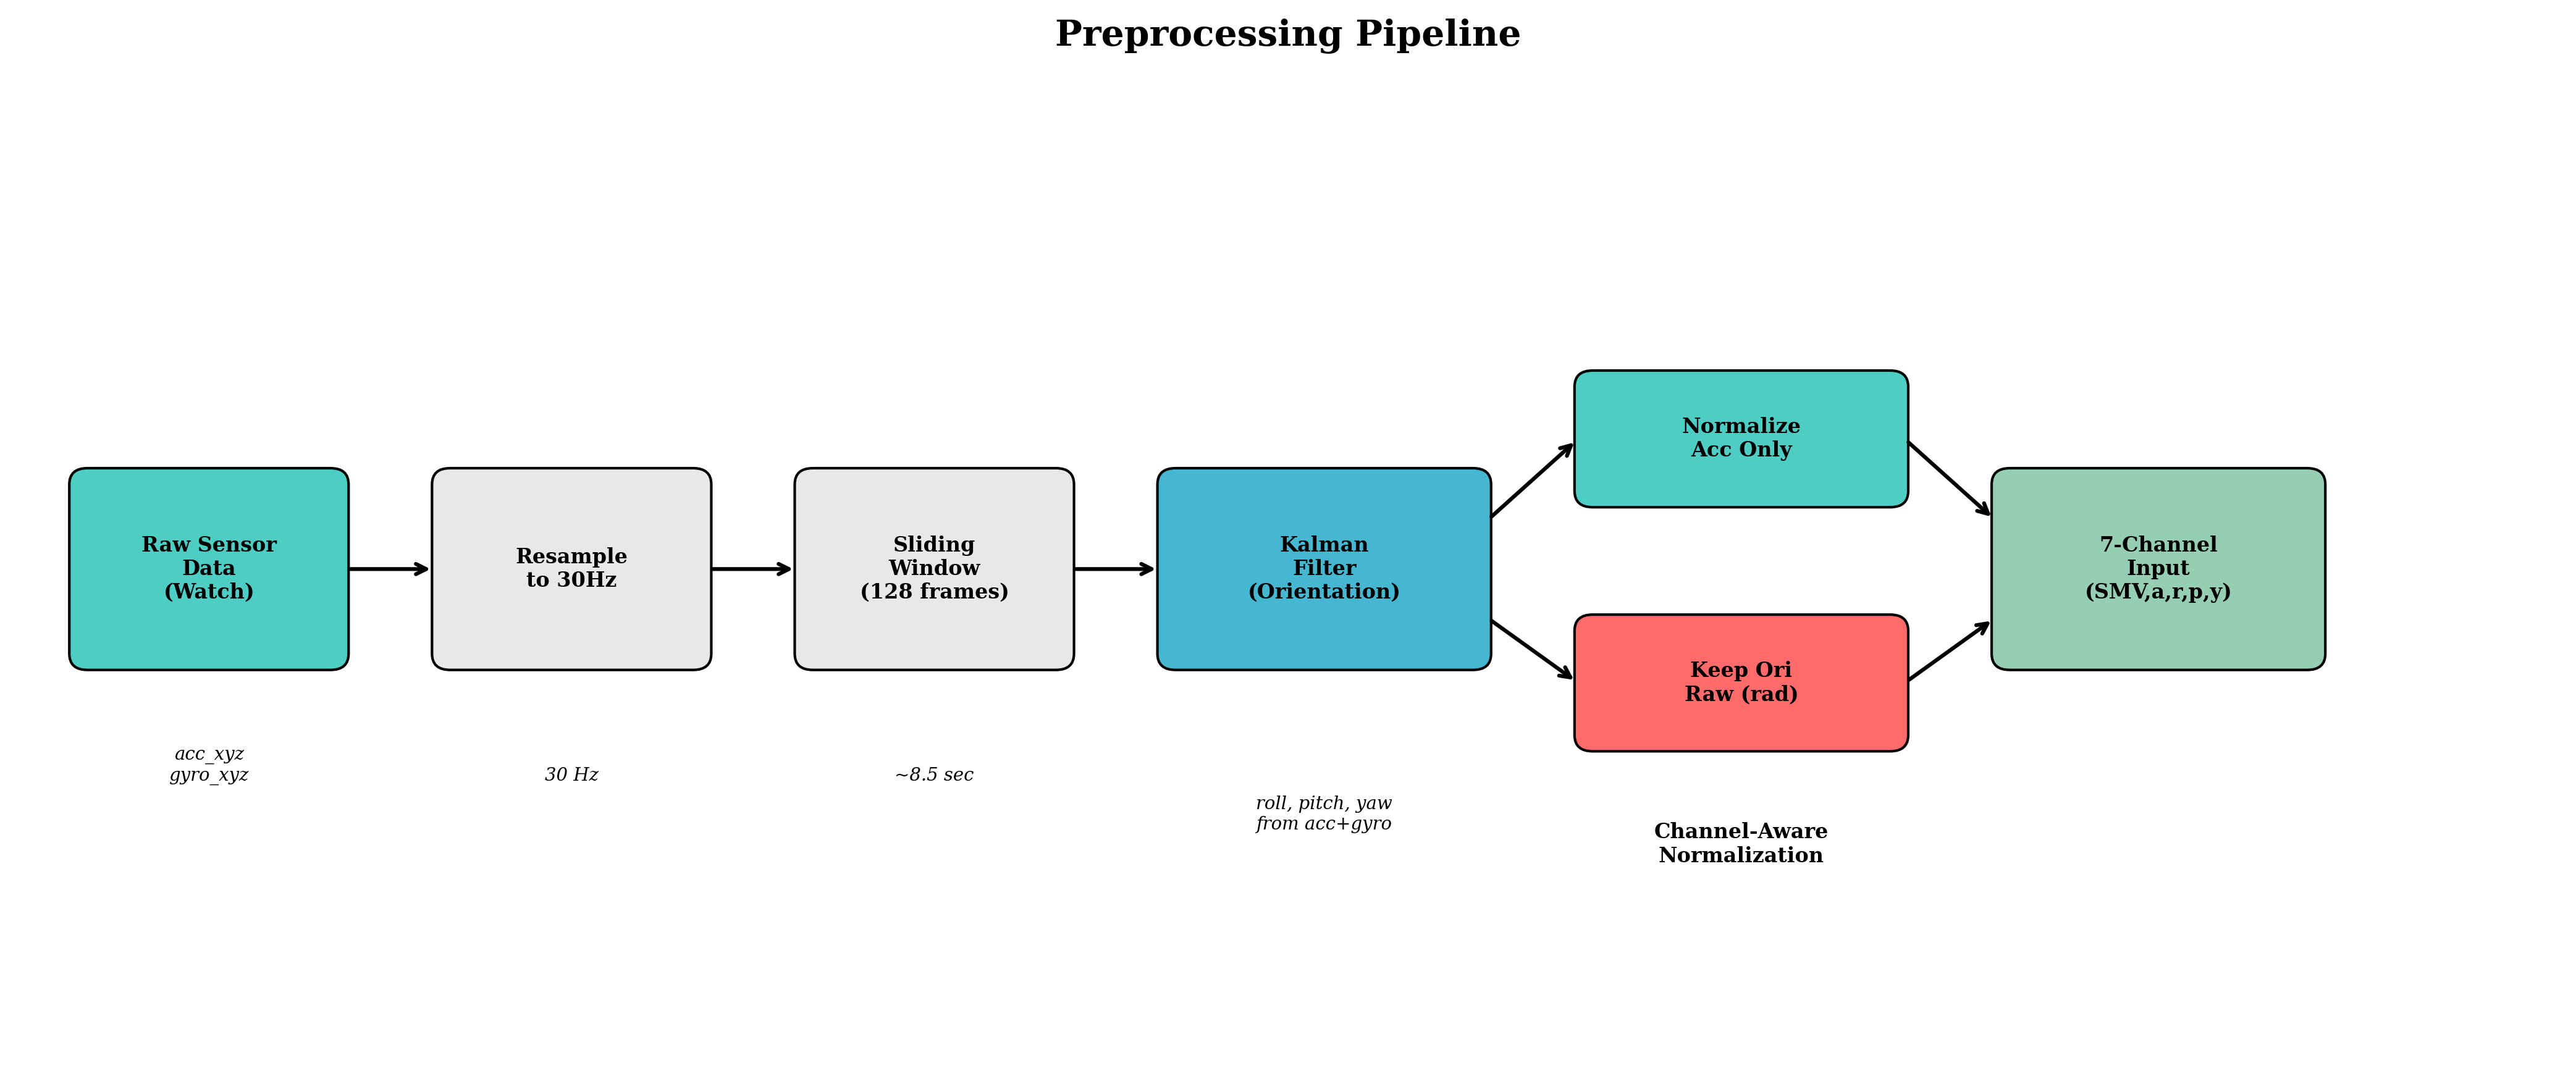
\includegraphics[width=0.9\columnwidth]{figures/preprocessing_pipeline_detailed.png}
\caption{Preprocessing pipeline: raw IMU $\rightarrow$ Kalman fusion $\rightarrow$ channel-aware normalization $\rightarrow$ sliding window segmentation.}
\label{fig:preprocessing}
\end{figure}

\textbf{Stage 1: Unit Conversion.} Raw gyroscope readings are converted from degrees/s to radians/s:
\begin{equation}
\boldsymbol{\omega}_{\text{rad}} = \boldsymbol{\omega}_{\text{deg}} \cdot \frac{\pi}{180}
\end{equation}

\textbf{Stage 2: Kalman Fusion.} The 6-channel raw input $[\mathbf{a}, \boldsymbol{\omega}] \in \mathbb{R}^{T \times 6}$ is transformed to 7 channels:
\begin{equation}
\mathbf{X} = [\text{SMV}, a_x, a_y, a_z, \phi, \theta, \psi] \in \mathbb{R}^{T \times 7}
\end{equation}
with Kalman parameters: $Q_{\text{ori}}{=}0.005$, $Q_{\text{rate}}{=}0.01$, $R_{\text{acc}}{=}0.05$, $R_{\text{gyro}}{=}0.1$.

\textbf{Stage 3: Channel-Aware Normalization.} We apply z-score normalization \textit{only} to accelerometer channels:
\begin{equation}
\tilde{x}_i = \begin{cases}
(x_i - \mu_i) / \sigma_i & \text{if } i \in \{0,1,2,3\} \text{ (acc)} \\
x_i & \text{if } i \in \{4,5,6\} \text{ (orientation)}
\end{cases}
\end{equation}
This preserves the physical meaning of orientation angles (bounded in $[-\pi, +\pi]$ rad), while normalizing unbounded accelerometer values that can spike to 30+ m/s$^2$ during falls.

\textbf{Stage 4: Sliding Window.} Sequences are segmented with window size $W{=}128$ samples ($\approx$4.3s) using class-aware strides:
\begin{equation}
s = \begin{cases}
16 \text{ samples} & \text{(fall windows)} \\
64 \text{ samples} & \text{(ADL windows)}
\end{cases}
\end{equation}
The asymmetric stride generates more fall training examples to address class imbalance.

\subsection{Evaluation Protocol}
\label{sec:Evaluation}

We employ rigorous Leave-One-Subject-Out Cross-Validation (LOSO-CV) to evaluate generalization to unseen individuals, which is critical for real-world deployment. This section details our protocol to ensure reproducibility and address potential concerns about data leakage.

\subsubsection{Subject Allocation}

The SmartFallMM dataset contains 51 subjects with asymmetric activity coverage:

\begin{itemize}
\item \textbf{Young subjects (30)}: Ages 18--35, performed both falls (5 types $\times$ 3--5 trials) and ADLs (8 types $\times$ 3--5 trials). These subjects can be tested on fall detection.
\item \textbf{Elderly subjects (21)}: Ages 65+, performed only ADLs due to safety constraints prohibiting induced falls. These subjects contribute ADL samples for training only.
\end{itemize}

Of the 30 young subjects, 2 are reserved as a fixed validation set (subjects 48, 57, selected for data completeness), and 7 have incomplete data due to sensor failures or protocol deviations. This yields \textbf{21 testable young subjects} for LOSO-CV evaluation.

\subsubsection{LOSO-CV Protocol}

For each fold $i \in \{1, \ldots, 21\}$:
\begin{enumerate}
\item \textbf{Test set}: All samples from young subject $S_i$ (both falls and ADLs)
\item \textbf{Validation set}: Fixed subjects [48, 57] (never appear in any test fold)
\item \textbf{Training set}: All elderly subjects (21) + remaining young subjects (excluding $S_i$, 48, 57)
\end{enumerate}

This protocol ensures complete subject-level separation: no sample from the test subject appears in training, and no sample from validation subjects appears in any test fold.

\subsubsection{Hyperparameter Tuning Strategy}

We use \textit{global hyperparameter tuning} with frozen parameters across all LOSO folds, following the methodology of Cawley and Talbot~\cite{cawley2010overfitting}:

\begin{enumerate}
\item \textbf{Tuning phase}: Grid search over learning rate $\in \{10^{-4}, 5{\times}10^{-4}, 10^{-3}, 5{\times}10^{-3}\}$, dropout $\in \{0.3, 0.4, 0.5, 0.6\}$, and embedding dimension $\in \{32, 64, 128\}$, evaluated on the fixed validation set.
\item \textbf{Evaluation phase}: Selected hyperparameters (lr$=$0.001, dropout$=$0.5, embed\_dim$=$64) are frozen for all 21 LOSO folds.
\end{enumerate}

This prevents hyperparameter selection from introducing test information leakage while maintaining computational tractability (nested CV would require 21$\times$ grid search iterations).

\subsubsection{Windowing and Sample Independence}

Sliding window segmentation is applied \textit{after} subject-level splitting, ensuring zero cross-subject sample correlation:

\begin{enumerate}
\item Subject $S_i$ assigned to test set
\item Raw trials loaded per subject
\item Sliding windows ($W{=}128$, stride 16/64) created \textit{within} each split
\end{enumerate}

Windows from subject $S_{49}$ (training) cannot overlap with windows from subject $S_{50}$ (test) because they derive from physically separate recordings. Within-subject window correlation is expected and does not constitute leakage---the model must still generalize to unseen subject $S_{50}$'s motion patterns.

\subsubsection{Evaluation Metrics}

We report F1 score as the primary metric due to class imbalance (falls are rare events), along with accuracy, precision, and recall. All results report mean $\pm$ standard deviation across the 21 LOSO folds. Statistical comparisons use paired $t$-tests across fold-level F1 scores.

